\documentclass[a4paper,UTF8]{article}
\usepackage{ctex}
\usepackage[margin=1.25in]{geometry}
\usepackage{color}
\usepackage{graphicx}
\usepackage{amssymb}
\usepackage{amsmath}
\usepackage{amsthm}
%\usepackage[thmmarks, amsmath, thref]{ntheorem}
\theoremstyle{definition}
\newtheorem*{solution}{Solution}
\newtheorem*{prove}{Proof}
\usepackage{multirow}
\usepackage{url}
\usepackage[colorlinks,urlcolor=blue]{hyperref}
\usepackage{enumerate}
\renewcommand\refname{参考文献}


%--

%--
\begin{document}
\title{\textbf{《计算机图形学》 6月报告}}
\author{161220062 李奡程 \href{mailto:xxx@xxx.com}{161220062@smail.nju.edu.cn}}
\maketitle

\section{综述}
\paragraph{完成的内容} 完成了全部大作业内容,包括线元、多边形、椭圆和两种曲线的生成,上述图元的平移、旋转、缩放和线段的裁剪,并在前后端分离的基础上分别开发了命令行界面和图形界面。
\section{算法介绍}
\subsection{线画图元介绍}
\paragraph{Digital Differential Analyzer} 数字差分分析,每次根据斜率在一个坐标轴上以单位间隔对线段取样($\Delta x=1$或$\Delta y=1$),据其计算另一个坐标轴上最靠近线段路径对应的整数值,以此作为最后生成的线元的整点\cite{graphTextBook}。记斜率为$m$,若$|m|>1$,则对于间隔$\Delta x=1$,顺序y值可计算为:
\begin{equation}
y_{k+1}=y_k+m
\end{equation}
对$|m|\leq 1$类似有
\begin{equation}
x_{k+1}=x_k+\frac{1}{m}
\end{equation}
\par 然而,实际实现时,可能存在直线垂直于x轴或y轴的情况,我采用的办法是特殊处理,保证斜率取值合法再进行DDA,否则只用在某一条平行线上赋值,这样的话存在高效存取方法实现。
\paragraph{Bresenham算法} 详细算法课本上有,所以在此用我的语言归纳总结一下,其针对DDA中可能出现的累积误差的问题,选择使用决策函数来在每一点决定下一个点时的选择,并通过动态更新决策函数有力的消除了累计误差的问题,而且其全部使用整数计算,开销比全部使用浮点数的DDA大大减少。
\par 具体的,对于第一象限的直线,斜率小于1时,在点$(x_k,y_k)$处,$p_k$的更新公式为
\begin{equation}
p_{k+1}=\left\{
\begin{array}{ll}
p_k+2\Delta y-2\Delta x & p_k>0 \\
p_k+2\Delta_y & p_k<0 \\
\end{array}
\right.
\end{equation}
且初始化其为
\begin{equation}
p_0=2\Delta y-\Delta x
\end{equation}
而对于其他象限以及其他斜率的直线,可对应变换$x$,$y$,$p_k$的相应项完成。由于象限间的对称性,在我实现中通过规定$y$的相对关系将需要处理的情况减为4种,再通过对称性仅处理两种情况即可。
\paragraph{测试}
\begin{figure}
	\centering
	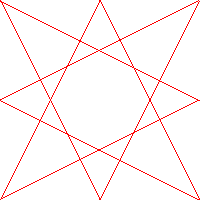
\includegraphics[height=6cm]{1.png}
	\caption{Bresenham 测试图样}
	\label{testLine}
\end{figure}
由于Bresenham需要处理8种情况,所以应该使测试用例覆盖8个朝向的边保证正确地覆盖所有可能。我使用了图\ref{testLine}中的八条线来检测,其结果清晰可见,并且能很快的显示出错误的可能原因,加速了我的debug过程。上图也用于检测DDA的实现的正确性。
\subsection{多边形}
\paragraph{绘制} 由于多边形可以视为由若干条直线构成,所以在此我复用线的相关算法,将多边形的各个边画分别画好即完成绘制。注意到多边形接受输入时可能有重点,所以处理时特判即可。
\subsection{椭圆}
\paragraph{中点圆生成算法} 即为Bresenham算法,借鉴Bresenham累积误差的思想,以及利用椭圆的对称性,通过第一象限中分割为斜率的绝对值小于1的两部分,并在各部分通过一边每次加一、另一边用判断函数决定位置来减少累积误差。以下讨论第一象限的处理情况,设曲线解析式为$\frac{x^2}{a^2}+\frac{y^2}{b^2}=1$,且$a>b$,则使用齐次坐标时该曲线表示为\cite{homographyBook}
\begin{equation}
\mathbf{C}=\left(
\begin{array}{ccc}
b^2 & 0 & 0 \\
0 & a^2 & 0 \\
0 & 0 & -a^2b^2 \\
\end{array}
\right)
\end{equation}
其中$\mathbf{C}$满足$\mathbf{x}^T\mathbf{C}\mathbf{x}=0$。由参考书知,曲线C在某一点$\mathbf{x}=(x_0,y_0,1)^T$处的切线即为$\mathbf{Cx}$,使该点斜率为1,可得
\begin{equation}
b^2x_0=a^2y_0
\end{equation}
带回曲线解析式,可得交点坐标为$(\frac{a^2}{\sqrt{a^2+b^2}},\frac{b^2}{\sqrt{a^2+b^2}})$,即在$0\leq x\leq x_0$段上,y的斜率的绝对值恒小于1,故每次增加x判断y;在$x_0\leq x\leq a$段上,y的斜率的绝对值恒大于1,故每次减少y判断x。
\par 而对于第一部分,我们使用椭圆决策函数判断,其表达式为\cite{graphTextBook}
\begin{equation}
p_{1k}=f_{ellipse}(x_{k+1},y_k-\frac{1}{2})=b^2(x_k+1)^2+a^2(y_k-\frac{1}{2})^2-a^2b^2
\end{equation}
若$p_{1k}<0$,则中点位于椭圆内,$y_{k+1}=y_{k}$不变;反之则$y_{k+1}=y_k-1$。联立,可得判断条件为
\begin{equation}
\left\{
\begin{array}{ll}
p_{1k+1}=p_{1k}+2b^2x_k+3b^2 & p_{1k}<0 \\
p_{1k+1}=p_{1k}+2b^2x_k-2a^2y_k+2a^2+3b^2 & p_{1k}\geq 0 \\
\end{array}
\right.
\end{equation}
\par 对于区域2,此时决策函数变为
\begin{equation}
p_{2k}=f_{ellipse}(x_{k}+\frac{1}{2},y_k-1)=b^2(x_k+\frac{1}{2})^2+a^2(y_k-1)^2-a^2b^2
\end{equation}
同时相应修改判断条件。得到第一象限表示后,将其对称投影到剩下三个象限,即得到最后的椭圆。
\subsection{曲线}
\paragraph{Bezier曲线} 一般曲线曲面采用参数表示,在以下的讨论中都假设参数为$u$,且$u\in[0,1]$。Bezier曲线使用Berstein基函数作为其基础,将$n+1$个控制点的曲线转为$n$次曲线表示,其中Berstein基函数形式为
\begin{equation}
BEZ_{i,n}(u)=\left(
\begin{array}{c}
n \\
i \\
\end{array}
\right)u^i(1-u)^{n-i}
\end{equation}
而曲线形式为
\begin{equation}
P(u)=\sum_{i=0}^{n}P_iBEZ_{i,n}(u), u\in[0,1]
\end{equation}
\par 由于Bezier曲线基函数实际为$(u+(1-u))^n$的二项式展开,其具有许多直接的数学变换公式,如降阶公式\cite{graphTextBook}
\begin{equation}
BEZ_{i,n}(u)=(1-u)BEZ_{i,n-1}(u)+uBEZ_{i-1,n-1}(u)
\end{equation}
就是由
\begin{equation}
\left(
\begin{array}{c}
n \\
i \\
\end{array}
\right)=
\left(
\begin{array}{c}
n-1 \\
i \\
\end{array}
\right)+
\left(
\begin{array}{c}
n-1 \\
i-1 \\
\end{array}
\right)
\end{equation}
推导而来,所以其具有很多优良性质,如端点位置、对称性、仿射不变性、凸包性、直线再生性、保型性等,但是其只具有拟局部性,对于局部调整,还是会引起全局的变化。由于其基函数中为二项式展开,所以组合中的很多公式都可以直接应用,并作为降阶公式简化计算。在我的实现中,直接计算相应的Bezier矩阵,利用连续性的边界条件得到其通式,计算出n阶的Bezier矩阵,并在参数域上等间距选择$u$点的位置算出矩阵乘积(使用公式6-198\cite{graphTextBook})作为最后输出。
\par 同时也可以采用de Casteljau递推算法产生曲线上的点,其原理类似初始的降阶公式,形式为
\begin{equation}
P_i^{r}=\left\{
\begin{array}{ll}
P_i & r=0 \\
(1-u)P_i^{r-1}+uP_{i+1}^{r-1} & r=1,2,\ldots,n; i=0,1,2,\ldots,n-r \\
\end{array}
\right.
\end{equation}
通过递归计算,得到$r=n$时的型值点,其即为真实曲线上的一点,且分割成两个更小的子曲线,可分别递归计算。
\paragraph{B样条曲线}
B样条曲线思路类似Bezier曲线,但是将基函数换为了更强的B样条基函数,并显示地设定了曲线的次数$k$,将参数曲线作节点分割形成不同的曲线,而B样条基函数只在参数区间中分段连续有值,故能保证局部性。其具体形式为(使用deBoox-Cox递推公式)\cite{graphTextBook}
\begin{equation}
B_{i,k}(u)=[\frac{u-u_i}{u_{i+k-1}-u_i}]B_{i,k-1}(u)+
[\frac{u_{i+k}-u}{u_{i+k}-u_{i+1}}]B_{i+1,k-1}(u), i=0,1,2,\ldots,n
\end{equation}
其中基条件为
\begin{equation}
B_{i,u}=\left\{
\begin{array}{ll}
1 & u\in[u_{i},u_{i+1}] \\
0 & otherwise \\
\end{array}
\right.
\end{equation}
则对于$n+1$个控制顶点$\mathbf{P}=\{P_i|i=0,1,\ldots,n\}$,参数节点向量$U_{n,k}=\{u_i\}$,k阶B样条曲线形式为
\begin{equation}
P(u)=\sum_{i=0}^{n}P_iB_{i,k}(u), u\in[u_{k-1},u_{n+1}]
\end{equation}
B样条曲线具有局部性、凸包性、直线再生性、分段参数多项式曲线性、连续性、仿射不变性、平面曲线的保型性等优良性质。在我的实现中,通过递归计算$B_{i,k}(u)$的取值,可以通过遍觅参数区间得到最终的曲线点集,从而绘制B样条曲线。
\par 由上述讨论可以看出曲线的阶数k和参数节点向量对于最终形成的曲线有重要影响,而且根据不同的参数节点构成形成了不同类型的B样条曲线,如均匀B样条曲线是由均匀划分参数轴的节点向量构成,通过使向量中两端节点具有重复度k+1,可以构成准均匀B样条曲线,在这种情况下其会通过控制顶点集的两端。在我的实现中,使用的是均匀B样条曲线。
\subsection{图元的平移}
\paragraph{原理} 图元的平移等操作属于图形观察和变换中的一部分,其描述了一个物体应该怎么样转换到另一个坐标系中表示,并且高效地在不同坐标系间建立转换关系。不同于课本,在此我使用常用的齐次坐标表示方法来解释这部分的转换关系。
\par 由于这次实现的是二维系统的变换,实际上普通的加上偏移量作为平移就足够,但是为了表示的完整性,在这里采用齐次矩阵(Homography)的形式描述,故平移$(t_x,t_y)$可以表示为
\begin{equation}
\left(
\begin{array}{c}
x_2 \\
y_2 \\
1 \\
\end{array}
\right)
=\left(
\begin{array}{ccc}
1 & 0 & t_x \\
0 & 1 & t_y \\
0 & 0 & 1 \\
\end{array}
\right)
\left(
\begin{array}{c}
x_1 \\
y_1 \\
1 \\
\end{array}
\right)
\end{equation}
在实际计算中,可以将原来非齐次坐标下的加法变为乘法,从而形成仿射变换群,可以存储多个变化至同一处,方便整体的表示与计算。
\paragraph{图元的处理} 由于目前的各个图元都具有仿射不变性,所以在二维变换下可以通过直接将相应的控制点作相应的齐次变换后构造新图元即可,比如线段可以通过平移两边的端点,再在新位置上画出相应图元;椭圆平移圆心即可;多边形则对每一段直线都做相应处理即可;Bezier曲线和B样条曲线由于其放射不变性,所有变换都可以通过直接作用到其控制点集上后再重新绘制获得新图元。
\par 由于平移后可能出现超出边界的情况,而若在各个图元上添加裁剪操作的支持较为困难,所以在这里我采用保守策略,即检测到可能超出边界的图元时会终止平移操作,并报告越界错误。
\subsection{图元的旋转}
\paragraph{原理} 图元的旋转同样可以通过齐次矩阵表示,计算出其与旋转中心的差值后再平移回相应位置,过程可以表示为\cite{homographyBook}
\begin{equation}
\left(
\begin{array}{c}
x_2 \\
y_2 \\
1 \\
\end{array}
\right)
=
\left(
\begin{array}{ccc}
1 & 0 & t_x \\
0 & 1 & t_y \\
0 & 0 & 1 \\
\end{array}
\right)
\left(
\begin{array}{ccc}
\cos\theta & -\sin\theta & 0 \\
\sin\theta & \cos\theta & 0 \\
0 & 0 & 1 \\
\end{array}
\right)
\left(
\begin{array}{ccc}
1 & 0 & -t_x \\
0 & 1 & -t_y \\
0 & 0 & 1 \\
\end{array}
\right)
\left(
\begin{array}{c}
x_1 \\
y_1 \\
1 \\
\end{array}
\right)
\end{equation}
\paragraph{图元的处理} 由于旋转变换仍属于仿射变换群,而所有的图元都是仿射不变的,所以仍然通过计算其控制点旋转后的位置,再更新图元即可。未要求实现椭圆的旋转,如果要实现,可能需要更改椭圆的存储方式。
\subsection{图元的缩放}
\paragraph{原理} 缩放即比例变换,相对于定点的缩放可以通过先将其平移到原点,进行比例变换,最后再平移回相应距离完成,使用齐次坐标可以表示为(由于需求是恒等比例变换,所以$S_x=S_y=s$)
\begin{equation}
\left(
\begin{array}{c}
x_2 \\
y_2 \\
1 \\
\end{array}
\right)
=
\left(
\begin{array}{ccc}
1 & 0 & t_x \\
0 & 1 & t_y \\
0 & 0 & 1 \\
\end{array}
\right)
\left(
\begin{array}{ccc}
s & 0 & 0 \\
0 & s & 0 \\
0 & 0 & 1 \\
\end{array}
\right)
\left(
\begin{array}{ccc}
1 & 0 & -t_x \\
0 & 1 & -t_y \\
0 & 0 & 1 \\
\end{array}
\right)
\left(
\begin{array}{c}
x_1 \\
y_1 \\
1 \\
\end{array}
\right)
\end{equation}
\paragraph{图元的处理}
由于缩放仍属于仿射变换群,所以对所有图元仍然通过将其关键点缩放后重画获得新图元。另外缩放不会改变椭圆的长短轴角度,故可以正常实现。
\subsection{线段裁剪}
\paragraph{Cohen-Sutherland算法}
线段裁剪,其目的是获得线段在某一观察窗口内的情况,故裁剪后的线段可能被完全保留、部分保留或者完全丢弃。Cohen-Sutherland算法通过对观察窗口坐标系进行区域编码,快速判断线段与窗口间的关系,从而减少求交次数,加快裁剪速度。
\par 根据线段与窗口之间的大小关系,将平面分割为9个小平面,从左上开始分别编码为1001、1000、1010、0001、0000、0010、0101、0100、0110,四位中的每一位表示线段和窗口的左右上下的大小关系(以下简记为LRTB),则易见若两个端点区域码均为0000,则线段完全在窗口内;若两端点区位码的与不为0000,则必然完窗口外;对于其他情况,根据为1的位的相关信息,可以有效地找到需要求交的边,递归进行获得最终结果\cite{graphTextBook}。详细算法流程见图3-12,但是个人感觉直接使用递归求解代码更简洁。
\paragraph{梁有栋-Barsky算法}
梁有栋-Barsky算法从另一个角度处理裁剪问题,并将原问题的复杂性归因为裁剪窗口和线段的维数不同,并建议通过参数化表示线段,并获得裁剪窗口在线段所在直线上的交的位置的参数来判断是否需要裁剪。这种方法能够减少求交次数,并且最终获得的相交的参数即是最终裁剪线段的两端的端点的参数表示。
\par 设原线段两端端点位$P_1$和$P_2$,诱导窗口的交点坐标为$u_1$和$u_2$,则$P_1P_2$部分可见的充要条件为
\begin{equation}
\max(0,u_1)\leq \min(u_2,1)
\end{equation}
且可见区间就是$[\max(0,u_1),\min(u_2,1)]$。
\par 故高效的寻找裁剪窗口与线段的交的参数表示成为算法关键。梁有栋-Barsky算法采用的参数$p$和$q$分别为
\begin{equation}
\left\{
\begin{array}{ll}
p_1=\Delta x & q_1=x_1-x_{left} \\
p_2=-\Delta x & q_2=x_{right}-x_1 \\
p_3=\Delta y & q_3=y_1-y_{bottom} \\
p_4=-\Delta y & q_4=y_{top}-y_1 \\
\end{array}
\right.
\end{equation}
可以看出$p_i$表征线段和裁剪窗口边界的关系,若等于零,则平行于边界,大于0则从内部长到外部,小于0则从外部长到内部,并且交点即为
\begin{equation}
u=\frac{q_i}{p_i}
\end{equation}
可利用该u值反复更新$u_1$和$u_2$,直到稳定,即得到最后结果,再根据可见的充要条件进行保留、裁剪或舍弃\cite{graphTextBook}。
\subsection{命令行部分使用其他算法}
以上各小节介绍了各种图元的生成的设备级算法和其变换操作的原理,但是在实际使用中还有别的需要考量的部分,本节简述在命令行部分涉及的部分其他算法。
\paragraph{输入分析——简易Parser} 由于命令行需要接受输入,并且能够分析输入,所以我们需要自行设计一个简易的编译器来完成。由于输入完全可以由空格拆分关键词区分,所以我设计的简单Parser即通过获取每行第一个关键词,再根据关键词查表分析输入,最后接受输入并传给画图端或者拒绝并显示错误信息,提供较好的交互性。
\paragraph{画图——坐标变换} 为实现存储图元功能,我使用了opencv,其imwrite函数能快速将数组存储为bmp格式的图像,但是opencv的坐标和画图坐标不同:其x轴为y轴的逆方向,而y轴为x轴,所以在每次实际画图前还需进行一次坐标变换:
\begin{equation}
\left(
\begin{array}{c}
x_2 \\
y_2 \\
1 \\
\end{array}
\right)
=\left(
\begin{array}{ccc}
0 & -1 & h \\
1 & 0 & 0 \\
0 & 0 & 1 \\
\end{array}
\right)
\left(
\begin{array}{c}
x_1 \\
y_1 \\
1 \\
\end{array}
\right)
\end{equation}
\subsection{图形界面部分使用其他算法}
本节简述在图形界面部分使用的其他算法。
\paragraph{输入分析——坐标变换}
在PyQt中,接受的鼠标事件的坐标是相对于界面左上角的,且其y轴对应于opencv下的x轴,x轴对应于opencv下的y轴,故从用户坐标系到画图坐标系仍需要变换,此时变换关系为
\begin{equation}
\left(
\begin{array}{c}
x_2 \\
y_2 \\
1 \\
\end{array}
\right)
=\left(
\begin{array}{ccc}
0 & 1 & 0 \\
1 & 0 & 0 \\
0 & 0 & 1 \\
\end{array}
\right)
\left(
\begin{array}{c}
x_1 \\
y_1 \\
1 \\
\end{array}
\right)
\end{equation}
\paragraph{图元选定}
在用户界面,我们可能需要用户指定对某一图元作平移、旋转或缩放操作,因此我们需要设计一种机制使得能够选定用户希望选中的图元。我的做法是在绘图过程中使每个类额外保存其画的节点,等到用户有点击事件时,遍觅每个图元,输出其到用户选中点之间的最短距离,当所有图元的最短距离的最小值仍大于阈值时(我设定的是10个像素),则未选中任何图元;反之,则选定最短距离的图元。
\par 这种算法在图元比较稀疏的时候比较有效,当图元比较稠密时可以考虑通过从选中点作bfs找到最近距离的有色点,将该点对应图元作为选中的图元。
\section{系统介绍}
\paragraph{命令行界面} 
\begin{figure}
	\centering
	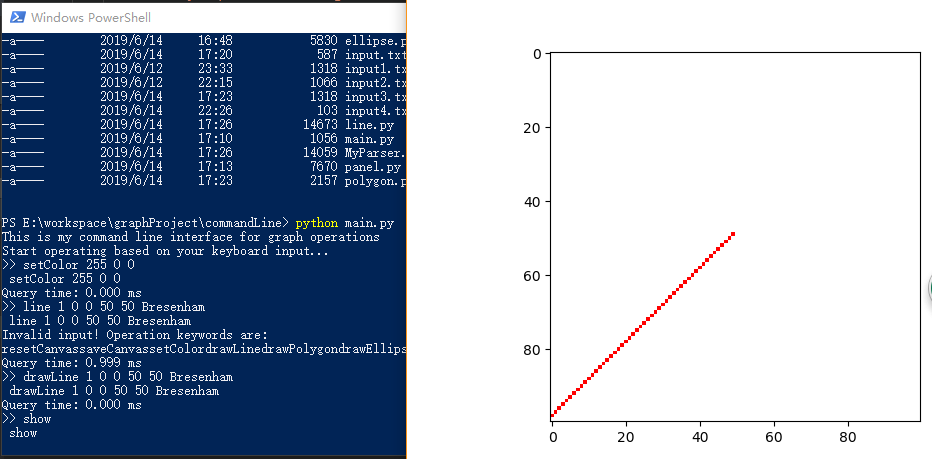
\includegraphics[height=8cm]{commandLineScrot.jpg}
	\caption{命令行运行实录}
	\label{commandLineLooklike}
\end{figure}
其分为命令行界面和图形界面两部分,分别位于两个文件夹下。命令行界面位于./commandLine 文件夹下,主要由四部分构成:
\subparagraph{main} 接收用户输入,显示相关信息;
\subparagraph{parser} 作为命令行前端,分析用户输入,进行基础的词法语法分析,拒绝非法输入,并将合法输入传到画图后端进行处理;
\subparagraph{panel} 其为画板,作为系统中间层,调用各种图元以完成各种图形操作,同时按照前端要求显示与保存图片。使用其作为中间层能够有效的屏蔽后端实现细节,并且直接作为GUI的中间层加以使用,而不用特别修改相应算法。
\subparagraph{各种图元} 受到sklearn中各种分类器、学习器类设计的启发,我意识到实际上可以将后端的功能进一步分离,设计好每种图元自身的数据结构,并使其支持draw,scale,rotate等操作(线段还要再支持clip操作),就可以直接通过panel保存图元字典来直接调用,在绘图时即遍觅字典使其调用draw函数,图元二维变换时也直接通过图元.rotate 类直接调用,从而实现更好的数据封装。目前相关实现在commandLine/Line.py,Polygon.py, Ellipse.py 和 Curve.py中,其为CLI和GUI共同的后端核心代码。
\subparagraph{库依赖与运行} 命令行部分为了实现画图和存图的功能,调用了python的库numpy, matplotlib 和opencv,需要安装这些库才能运行。运行在终端使用python main.py进行,目前可以在windows中运行,支持python3的版本。
\begin{figure}
	\centering
	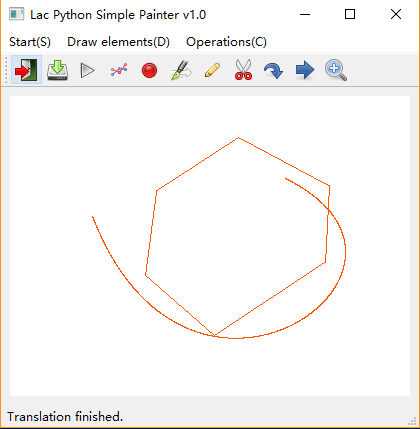
\includegraphics[height=8cm]{guiScrot.jpg}
	\caption{图形界面运行实录}
	\label{guiLooklike}
\end{figure}
\paragraph{图形界面} GUI部分位于./gui 文件夹下,使用PyQt完成,选择PyQt的原因是其提供了一个强大又易于开发GUI环境,并且同样使用python语言,能够兼顾之前书写的代码。其主要分为三部分:
\subparagraph{main} GUI的主窗口实现,包括各种交互界面,部件间的槽关系等;
\subparagraph{displayLabel} 重写后的QLabel类,其作为与用户交互的最前端,接受分析Mouse Press Event和Mouse Release Event获取用户输入,并传回main窗口进行相应操作,最后再将处理好的图片显示再QLabel上,完成整个交互过程;
\subparagraph{各种图元} 这里直接复用CLI中的相关部分,因为只需要调用它的接口,而不需对相关逻辑做出任何改动。
\subparagraph{库依赖与运行}
GUI部分除了和命令行部分相同的依赖于numpy, matplotlib 和opencv外,还需要PyQt5创建用户界面以运行。运行时同样使用python main.py,其不接受读入文件,而是直接通过图形界面进行交互。具体交互方法详见系统说明书。
\section{总结}
\paragraph{} 终于完成了整个画图项目,感觉还是收获颇多,首先是处理图像的能力,之前只是直接调用opencv中的函数cv.line或者cv.circle来画圆,从来没有认真考虑过后面的设备级生成算法是怎么来的,同时需要综合考虑各种算法的原理和其实现方法的不同,因为大部分算法是针对光栅扫描机制设计的,而我们实际操作的高级语言可能具有其他能够利用的特性,所以需要相应地对算法做出调整和改良,如在具有较多内存时可以存储所有的点来减少交互时的访存开销。
\par 课本上也有很多推导不完善甚至错误的地方,有些时候需要自己重新推导,虽然麻烦,但也确实加强了对相关内容的理解。
\par 另外通过对GUI的开发,我也深刻体会到图形学中很重要的一环:交互性,而且越是对用户来说优良的交互体验可能就越要耗费界面开发者的设计精力,
但一个友好的界面不仅对用户友好,也对开发者的开发过程友好,因为其能够有效提升测试效率,从而提升开发效率。另外目前只涉及了一些最基础的图像操作,以后希望有机会能使用更高级的操作方式来进行图形学系统的设计与开发。
\begin{thebibliography}{2019}
\bibitem{graphTextBook} 计算机图形学教程\quad 孙正兴主编\quad 周良,郑洪源,谢强编著
\bibitem{homographyBook} Multiple View Geometry in computer vision, Richard Hartley and Andrew Zisserman, Second Edition, 2004
\end{thebibliography}

\end{document}